\documentclass[exercice]{thedocument}%
\startdatakeys
\source{}
\cycle{}
\competencesDuSocle{}
\connaissancesRequises{}
\competencesTravaillees{}
\enddatakeys
\begin{document}%
\begin{minipage}[c]{.45\linewidth}
    Recopier et disposer dans le carré ci-contre les nombres entiers
    relatifs compris entre -8 et 7 tels que la somme de chaque ligne,
    de chaque colonne et de chaque diagonale soit toujours la même.
    Chaque nombre ne doit apparaître qu'une seule fois dans la grille.
\end{minipage}\hskip30pt minus 15pt
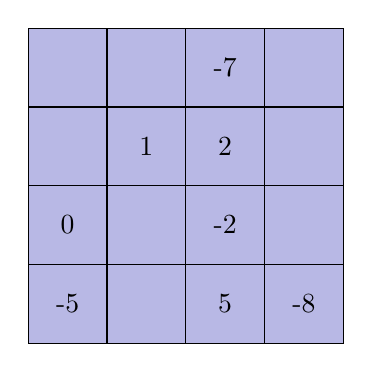
\begin{tikzpicture}[baseline=(current bounding box.center)]
    \draw[fill=blue!20!white!90!black](0,0)rectangle(4,4);
    \draw(0,1)--(4,1);
    \draw(0,2)--(4,2);
    \draw(0,3)--(4,3);
    \draw(1,0)--(1,4);
    \draw(2,0)--(2,4);
    \draw(3,0)--(3,4);
    \draw node at(0.5,0.5){-5};
    \draw node at(2.5,0.5){5};
    \draw node at(3.5,0.5){-8};
    \draw node at(0.5,1.5){0};
    \draw node at(2.5,1.5){-2};
    \draw node at(2.5,2.5){2};
    \draw node at(2.5,3.5){-7};
    \draw node at(1.5,2.5){1};
\end{tikzpicture}
\end{document}
